\documentclass[12pt]{article}
\usepackage{fullpage}
\usepackage{amsmath}
\usepackage{hyperref}
\usepackage{graphicx}
\usepackage{listings}
\usepackage{float}
\usepackage{alltt}

\floatstyle{plain}
\newfloat{snippet}{thb}{lop}
\floatname{snippet}{Snippet}

\newcommand{\mtt}[1]{\(#1\)}

\begin{document}
  \begin{center}
    \textbf{\large Out-of-Order SMIPS} \\
    6.375 Microarchitecture Design\\
    6 April 2011 \\
    
    \vspace{\baselineskip}
    
    \emph{Team}: David S. Greenberg and Bhaskar Mookerji
  \end{center}
  
  \begin{center}
      \textbf{Abstract}
  \end{center}
  \begin{quotation}
      For our 6.375 final project, we are implementing a out-of-order processor using Tomasulo's algorithm and 
      a reorder buffer. The following extends our high-level design to microarchitecture interfaces and 
      discusses an ROB entry tagging scheme that eliminates the need for content addressable memory.   
      
  \end{quotation}

\section{Tomasulo's Algorithm at a Glance}

Before getting into the details of Tomasulo's algorithm, let's try to understand it at a high level. An instruction set architecture (ISA) has a finite number of places in which
it can store variables. These places are called registers. Tomasulo's algorithm dynamically computes the dependencies between instructions so that instructions that
don't have data dependencies can run in parallel, while only the truly data-dependent instructions are run in sequence. This increases the throughput of the system by exploiting
instruction level parallelism (ILP). Tomasulo's algorithm can be seen as a dynamic hardware implementation of Static Single Assignment, a compiler technique that does
the same dependency calculations in software.

The core idea of Tomasulo's algorithm is that each ISA register has a corresponding physical register. Since instructions are dispatched in order but executed out of order,
we can associate the source operands of the instruction with the physical registers corresponding to the ISA registers used in the instruction. The destination register of
the instruction, however, is written to a new physical register, and the destination ISA register is updated to be linked to the new physical register. That way, every 
register is assigned once and only true dependencies affect execution.

Of course, hardware can't be allocated, and so Tomasulo's algorithm allocates the physical registers from a pool and releases registers back into the pool when there are
no more instructions using them as a source operand. The details of this are explained later.

\section{Problem\label{sec:problem}}
Although an elastic pipelined microprocessor is an improvement over an unpipelined processor, its performance suffers due to pipeline stalls.
There are three classes of stalls, two of which are eliminated by Tomasulo's algorithm.

The first class of stall is a Write-After-Read stall. This is where we see an instruction $A$ which reads from register $r_x$ followed by an instruction
$B$ which writes to the same register $r_x$. Normally, $B$'s execution is blocked by $A$ since they both need to access the same register. If $A$ has
several cycles of latency, then $B$ will be stalled until $A$ completes execution. Tomasulo's algorithm eliminates this false dependency by writing the
result of $B$ to a separate physical register, allowing $B$ to execute in parallel with $A$.

The second class of stall is a Write-After-Write stall. This is where we see an instruction $C$ which writes to a register $r_y$ followed by an instruction
$D$ which writes to the same register $r_y$. Normally, since both instructions need to write to the same ISA register, $D$ would be stalled until $C$ completed;
however, Tomasulo's algorithm allows them to execute in parallel since the instructions would each write to separate physical registers.

The third class of stall is a Read-After-Write stall, or a true data dependency. This is where instruction $E$ writes to register $r_z$, and then instruction $F$
reads from register $r_z$. Tomasulo's algorithm does nothing in this case, because since $F$ needs the result of $E$, it must be stalled until $E$ completes.

Let's look at an example snippet of code to understand an example situation in which Tomasulo's algorithm would help (Snippet~\ref{mulmovadd}).
In this simplified assembly language, the format of an instruction is $op$, $src_1$, $\left[src_2\right]$, $dst$; $src2$ is optional.

\begin{snippet}
\begin{verbatim}
mul r1, r2, r3
mov r3, r4
add r1, r2, r3
\end{verbatim}
\caption{Instruction sequence which would benefit from Tomasulo's algorithm}
\label{mulmovadd}
\end{snippet}

Let's assume that multiplies take 4 clock cycles, moves take 1 clock cycle, and adds take 2 clock cycles. Also, let's assume that fetching an instruction takes 1 clock cycle
and happens in parallel with execution. Then executing these instructions in sequence takes a total of 8 clock cycles--one cycle for the initial fetch, followed by each instruction
executing in sequence (Table~\ref{tab:simpleex1}). Since fetches are pipelined, we only see the fetch latency on the initial instruction. Now, if we are using Tomasulo's algorithm, we'll instead
see a total runtime of 6 clock cycles. To understand why, we can look at this table \ref{tab:tomasuloex1}.

\begin{table}
\begin{tabular}{l || c | c | c | c | c | c | c | c}
Cycle & 1 & 2 & 3 & 4 & 5 & 6  & 7 & 8 \\ \hline
Multiply & fetch & exec 1 & exec 2 & exec 3 & exec 4 & & \\
Move & & fetch & stall & stall & stall & exec & \\
Add & & & fetch & stall & stall & stall & exec 1 & exec 2 \\
\end {tabular}
\caption{Snippet \ref{mulmovadd} executed on a simply pipelined microprocessor}
\label{tab:simpleex1}
\end{table}

\begin{table}
\begin{tabular}{l || c | c | c | c | c | c}
Cycle & 1 & 2 & 3 & 4 & 5 & 6 \\ \hline
Multiply & fetch & exec 1 & exec 2 & exec 3 & exec 4 & \\
Move & & fetch & stall & stall & stall & exec \\
Add & & & fetch & exec 1 & exec 2 & \\
\end {tabular}
\caption{Snippet \ref{mulmovadd} executed on a microprocessor with Tomasulo's algorithm}
\label{tab:tomasuloex1}
\end{table}

\section{High-Level Design}

\begin{figure}[ht!]
    \centering
    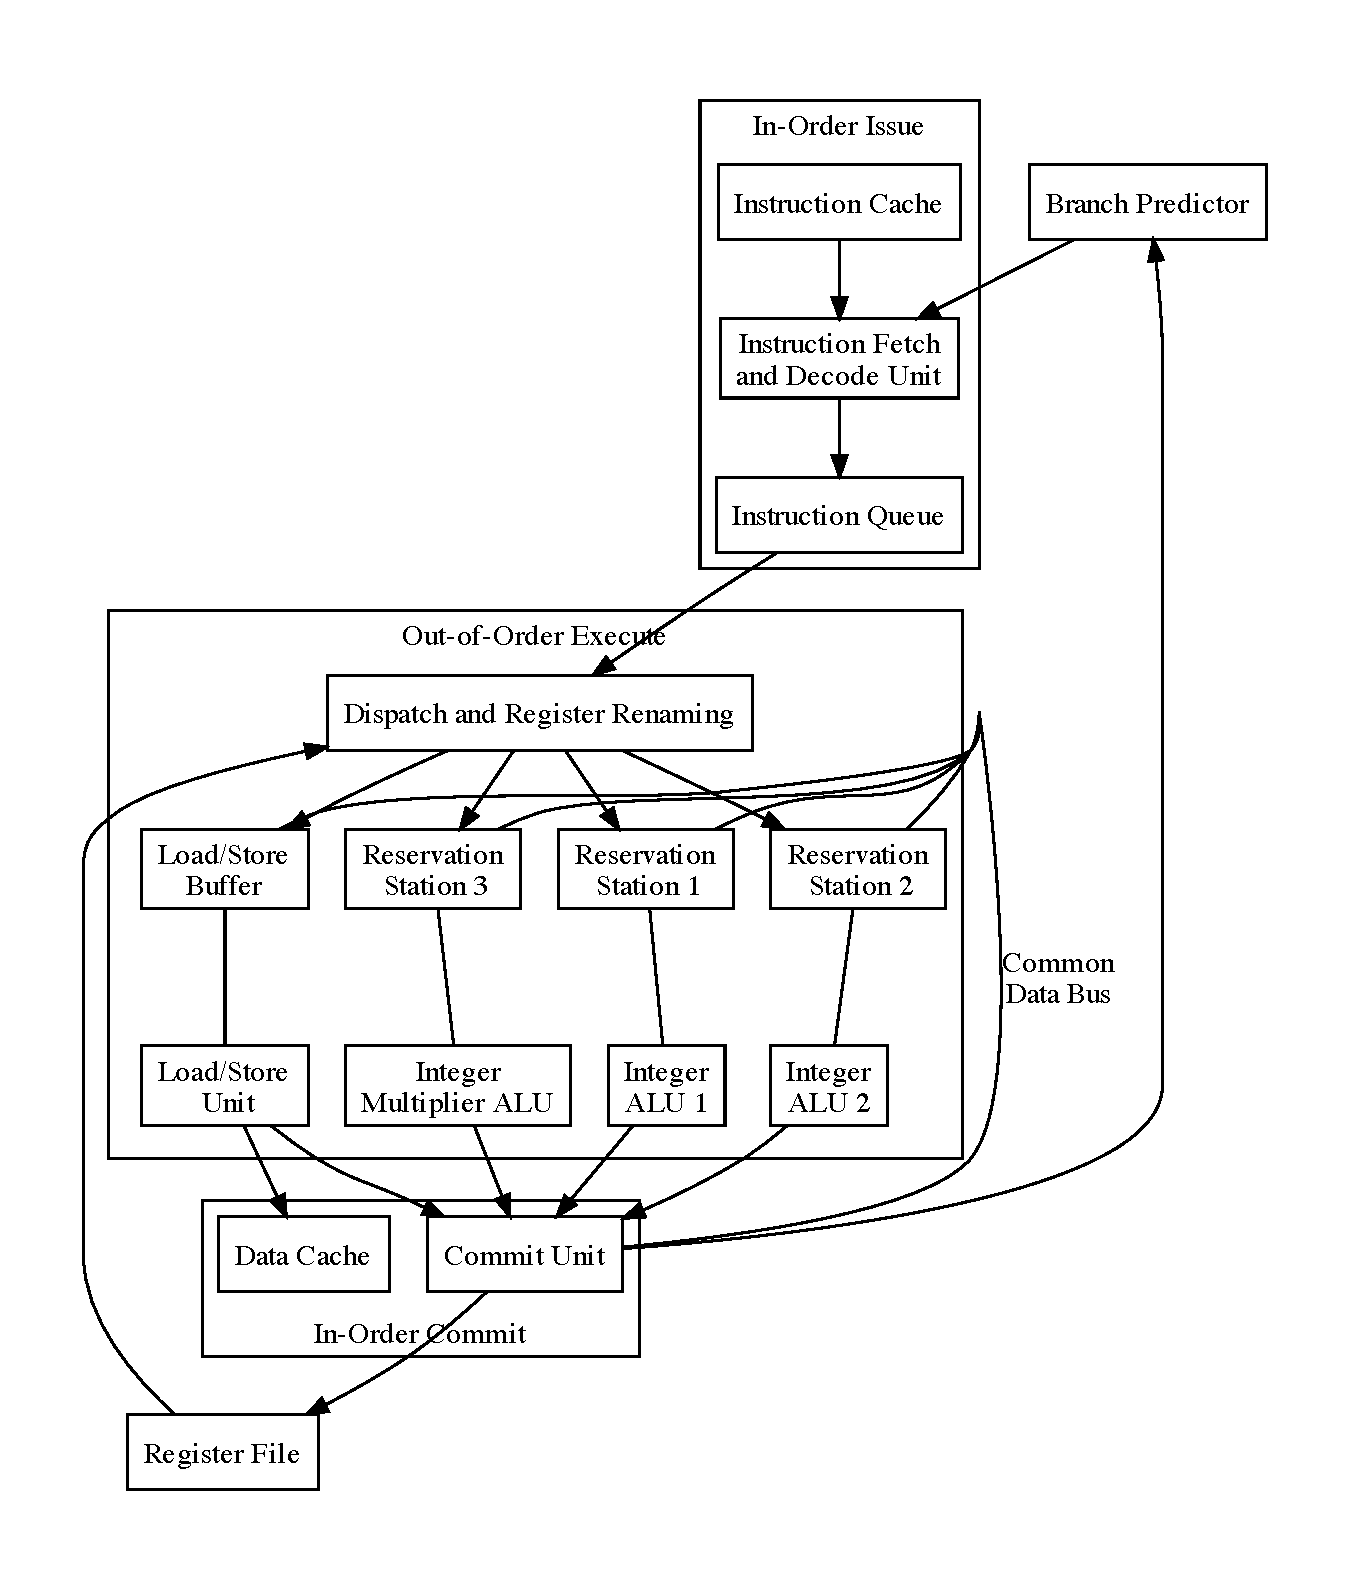
\includegraphics[width=\textwidth]{figures/design.pdf}
    \caption{System architecture using out-of-order execution and pipelined integer arthmetic. \label{fig:design}}
\end{figure}

\begin{figure}[h]
    \centering
    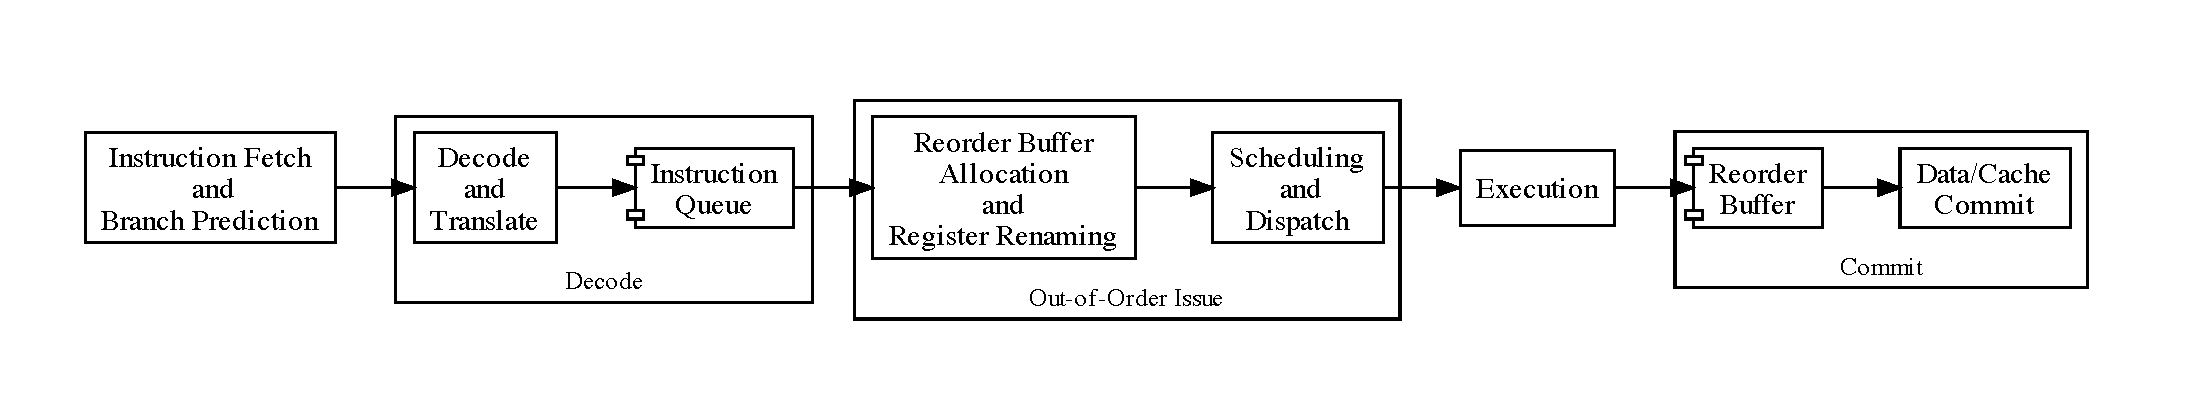
\includegraphics[width=1.1\textwidth]{figures/pipeline.pdf}
    \caption{Instruction pipeline. Pipeline stage is labeled in-box, unless superseded by an overbox. A component box indicates component (such as a FIFO) between stages. Not included in this diagram is the reservation stations and load/store buffer in the execution stage.\label{fig:pipeline}}
\end{figure}

The system design and instruction pipeline for our implementation is described
in Figure~\ref{fig:design} and~\ref{fig:pipeline}, respectively. 
The design extends our existing SMIPSv2 
implementation into three components: in-order instruction fetch and decoding, 
out-of-order execution units, and a commit unit. The instruction fetch and 
decode stage enqueues and dispatches instructions to reservation stations 
matching the appropriate execution unit, reordering as necessary to remove the 
pipelining hazards described in Section~\ref{sec:problem}. When the reservation 
station contains the appropriate operands for a given instruction, execution 
proceeds, and results are broadcast on a common data bus to waiting reservation 
stations and the branch prediction unit. The commit unit is implemented as a 
reorder buffer, and performs in-order commits to memory and the register file. 
Taken together with dispatch and register renaming, the reorder buffer and the 
reservation stations implement Tomasulo's algorithm.   

\section{Goals and Testing Strategy}

\subsection{Functional Correctness}

We will use the existing SMIPS implementation and toolchain to provide inputs, gather 
outputs, log rule executions as traces, and benchmark our implementation. Verifying the 
correctness of the Tomasulo's algorithm implementation will first require modular refinement
of fundamental components, such as the reorder buffer and reservation stations, before 
they are incorporated into our existing SMIPS implementation. To formally verify functional correctness,
we can examine traces for two different areas: data consistency invariants and instruction 
completion/termination/stalling conditions\footnote{This criteria for functional correctness in Tomasulo's
algorithm are described in greater detail in Chapter 6 of 
\emph{Design and Evaluation of a RISC Processor with a Tomasulo Scheduler} at~\url{http://www.kroening.com/diplom/diplom/}}.  

To further check for bugs, we will unit test with short programs that 
emphasize particular issues: sequences of dependent instructions, sequences of independent
arithmetic instructions, small loops, atypical branch sequences, and memory operations. 
Verifying the traces for these smaller test programs will simplify execution debugging 
for the existing benchmarks.

\subsection{FPGA Synthesis}
We've removed all CAM from the system, and so we believe that we should be able to 
synthesize modulo routing constraints.

\subsection{Performance}
Raw performance is not the goal of this project. With this architecture, we might not 
reach the IPCs of the three-stage pipeline architecture in Lab 4. To demonstrate the 
improvement of out-of-order execution in our processor, we will artificially introduce 
latency into our execution units using pipelined integer arithmetic routines. Theoretical 
performance and correctness are the primary concerns. Our design 
should enable future developers to use  a modularized Tomasulo's algorithm to hide the 
latencies of their additional instructions.
Unfortunately, there is way to show a strict benefit to the elastic pipelined SMIPS 
processor, since all ALU ops and multiplies  are single cycle on an FPGA anyway, and any 
worthwhile multicycle operation is a project in and of itself to implement.


\section{Microarchitecture Overview}

\subsection{New System Types}

To keep in-order instruction issue and retiring through the reorder buffer, we're introducing some new datatypes. 

\begin{enumerate}
    \item \textbf{Reorder Buffer Tag and Reorder Buffer Entry.} This is used to know which instruction (and thus its destination register) some piece of data corresponds to (could be an instruction or a result) in the reorder buffer. At instruction issue, this type is generated by a token request at the reorder buffer. Keeping track of this value eliminates the need for associative lookup. For ALU ops, stores the destination register, the Maybe\#(value), and the epoch of the instruction. For branch ops, stores the same stuff as the ALU ops and, if it was a mispredict, the correct address.
    \begin{alltt}
        typedef Bit#(4) ROBTag;
        
        typedef struct {
            Maybe#(Data) data;
            Maybe#(Tuple2(Addr,Addr)) mispredict;
            Rindx dest;
            Epoch epoch;
        } ROBEntry deriving (Bits, Eq);
    \end{alltt}
    \item \textbf{Reservation Station Entry.} This stores the reorder token it corresponds to, the operation to execute, and either the computed operands or the token that will contain their result. 
    \begin{alltt}
        typedef union tagged {
            ROBTag Tag;
            Data Value; // ugh
        } Operand deriving (Bits, Eq);
        
        typedef struct {
            InstrExt op;
            ROBTag tag;
            Bool full;
            Operand op1;
            Operand op2;
        } RSEntry deriving (Bits, Eq);
        
        typedef enum {ALU_OP, MEM_OP, JB_OP} Op_type deriving(Eq);    
    \end{alltt}
    \item \textbf{Common Data Bus Packet.} The CDB has the ROB token, execution value, and the Maybe\#(mispredict). 
    \begin{alltt}
        typedef struct {
            Maybe#(Data) data;
            ROBTag tag;
            Epoch epoch;
        } CDBPacket deriving (Bits, Eq);
    \end{alltt}
    \item \textbf{ALU Request and Response.}
    \begin{alltt}
        typedef struct {
            InstrExt  op;
            Data      op1;
            Data      op2;
            ROBTag    tag;
        } ALUReq deriving (Eq, Bits);

        typedef struct {
            Data   ans;
            ROBTag tag;
        } ALUResp deriving(Eq,Bits);
    \end{alltt}
\end{enumerate}

\section{Pipeline Stage Interfaces}
The pipeline stages, implemented as modules, are contained with a single processor module similar to the audio 
pipeline module from the earlier labs. The pipeline stages, connected by the appropriate FIFOs are:
\begin{enumerate}
    \item \textbf{Instruction Fetch}. Register address of operand $x$ is denoted by $x.A$.
        
    \item \textbf{Instruction Issue and Decode}.
       \begin{alltt}
           if (\mtt{\exists} free RS for \mtt{I\sb{i}} and !ROB.full):
               RS.op =  \mtt{I\sb{i}}
               RS.tag = ROB.tail
               
               \mtt{\forall} operands \mtt{x} of \mtt{I\sb{i}}:
                   if (\mtt{R\sb{x.A}} is Valid):
                       RS.op\mtt{\sb{x}} tagged Valid \mtt{R\sb{x.A}}.data
                   else if (CDB.tag == \mtt{R\sb{x.A}}.tag):
                       RS.op\mtt{\sb{x}} tagged Valid CDB.data
                   else if (ROB[\mtt{R\sb{x.A}}.tag] is Valid):
                       RS.op\mtt{\sb{x}} tagged Valid ROB[\mtt{R\sb{x.A}}.tag].data
                   else
                       RS.op\mtt{\sb{x}} tagged Invalid with \mtt{R\sb{x.A}}.tag
                       
               if (\mtt{I\sb{i}} has desination register \mtt{y.A})
                   \mtt{R\sb{x.A}}.tag = ROB.tail
                   ROB[ROB.tail].dest = \mtt{y.A}
               else
                   ROB[ROB.tail].dest = 0
       \end{alltt}
    \item \textbf{Dispatch}.
        \begin{alltt}
            \mtt{\forall} operands x
                if (RS.op\mtt{\sb{x}} tagged Invalid with .tag and tag == CDB.tag)
                    RS.op\mtt{\sb{x}} tagged Valid CDB.data
        \end{alltt}
    
        \begin{alltt}
            if (\mtt{\exists} free RS with Valid RS.op\mtt{\sb{x}} \mtt{\forall}
                operands x and !FU.stall):
                
                FU.op = RS.op
                FU.tag = RS.tag
                FU.op\mtt{\sb{x}} = RS.op\mtt{\sb{x}}
        \end{alltt}
        
    \item \textbf{Completion}.
        \begin{alltt}
            if (FU has result and got CDB-ack)
                CDB.data = FU.result
                CDB.tag = FU.tag
                
                ROB[CDB.tag] is tagged Valid CDB.data
        \end{alltt}
    \item \textbf{Graduate}.
        \begin{alltt}
            
        \end{alltt}
\end{enumerate}
The pipeline module interfaces are encapsulated as get/put servers and include the appropriate FIFOs. The connecting 
datatypes are described in greater detail in the next section.

\section{Architectural Interfaces}

\begin{enumerate}
    \item \textbf{Issue and Dispatch Units.} 
    \begin{itemize}
        \item[] Inputs: Instruction FIFO
        \item[] Outputs: Reservation Station Entry FIFO to the various execute units' reservation stations.
        \item[] Uses: Requests ROB token and places ROB entry, updates register map with the ROB token.
        \item[] Rules: If ROB token available and instruction ready, unpack instruction, fill in the known operands, 
        dispatch to a reservation station. If store instruction, wait for ROB to empty and issue.
    \end{itemize}
    
    \item \textbf{Reservation Stations.}
    \begin{itemize}
        \item[] Inputs: Reservation Station Entry FIFO
        \item[] Outputs: Send instruction to execute unit
        \item[] Rules: Snoops CDB and updating operands of held entries until they're ready, issuing instructions when 
        the operands are ready.
    \end{itemize}
    \begin{alltt}
        interface ReservationStation;
          method ActionValue#(RSEntry) getReadyEntry();
          method Action put(RSEntry entry);
        endinterface
    \end{alltt}
    
    \item \textbf{Common Data Bus.}
    \begin{itemize}
        \item[] Inputs: Put execution result (put with method Action)
        \item[] Outputs: execution result (multiple reader get (fanout)): all listeners must check the bus every cycle and never drop a packet
        \item[] Potential impl: Using bypass reg. for storing value, every listener must acknowledge before accepting a new value
    \end{itemize}
    
    \begin{alltt}
        interface CommonDataBus#(type t, numeric type nlisteners);
          method Action put(t entry);
          method ActionValue#(t) get(Bit#(TLog#(nlisteners)) id);
          method Bool hasData();
          method Action dumpState();
        endinterface
    \end{alltt}
    
    \item \textbf{ALU.}
    \begin{alltt}
        interface ALU;
            interface Server#(ALUReq, ALUResp) proc_server;
        endinterface
    \end{alltt}
    
    \item \textbf{Reorder Buffer.}
    \begin{itemize}
        \item[] Inputs: Listening to CDB, side effects of token requests
        \item[] Outputs: none
        \item[] Rules: graduate last instruction if it's been computed (includes writeback and removal from circular
        buffer), purge instructions of wrong epoch, issue a mispredict if a branch had been mispredicted, update the register map to use the architectural register for map entries whose token matches graduated instruction
    \end{itemize}
    \begin{alltt}
        interface ROB#(numeric type robsize);
          method ActionValue#(Bit#(TLog#(robsize))) reserve(ROBEntry robEntry);
          method Action update(Bit#(TLog#(robsize)) tag, ROBEntry robEntry);
          method Maybe#(ROBEntry) get(Bit#(TLog#(robsize)) tag);
          method ROBEntry getLast();
          method Action complete();
          method Bool isEmpty();
          method Bool isFull();
        endinterface
    \end{alltt}

    \item \textbf{Branch Predictor (BTB).} Available methods:
        \begin{itemize}
            \item[] Return what it would predict given its current state
            \item[] Speculate the next instruction
            \item[] Return that it mispredicted and needs to fix it
            \item[] Return the epoch.
        \end{itemize}

    \begin{alltt}
        interface BranchPredictor#(numeric type btbsize);
        	method ActionValue#(Addr) predict();
        	method Addr confirmPredict(Addr currentPc);
        	method Epoch currentEpoch();
        	method Action mispredict(Addr srcPc, Addr dstPc);
        endinterface
    \end{alltt}

\end{enumerate}

    \section{Implementation Status and Testing Plans}

      We have thus far implemented the ALU, the reservation stations, the common data (bypass) bus,
      the reorder buffer, and all of the system types. The common data bus and the reorder buffer have
      been unit tested for correctness. The branch predictor and memory subsystem have been ported,
      and the majority of Tomasulo's algorithm has been implemented. The load/store system must be
      still be implemented, and branch predictor and operand source search function must be tested.
      All 1322 lines of code compile without error.

    \section{Planned Design Exploration}
    
    We will explore architectural parametrization: 
    \begin{enumerate}
        \item Reorder buffer dimension
        \item Branch prediction strategies (BTB and 2-Bit)
        \item Register file bypassing and FIFO usage
        \item Multiple ALU instruction issue
        \item Artificial arithmetic and memory latency
    \end{enumerate}
    
    \section{Citations}
    

 \end{document}
